% flashcards-title: Power-of-ten scale
% flashcards-desc: A horizontal logarithmic scale has equal exponent steps from ten to the minus three through ten to the third. A striped marker P is at ten to the minus two and a gold marker Q is at ten to the first.
\documentclass[border=5mm]{standalone}
\def\pgfsysdriver{pgfsys-dvisvgm.def}
\usepackage{tikz}
\usetikzlibrary{arrows.meta,calc,patterns.meta,positioning}
\renewcommand{\familydefault}{\sfdefault}

\definecolor{fcInk}{HTML}{1C1C1E}
\definecolor{fcMuted}{HTML}{68686D}
\definecolor{fcGuide}{HTML}{C9C9CE}
\definecolor{fcGold}{HTML}{D7A313}
\definecolor{fcGoldSoft}{HTML}{F8E8AE}

\tikzset{
  fc canvas/.style={fill=white, rounded corners=2.5mm},
  fc vector/.style={
    draw=fcGold,
    line width=1.35mm,
    line cap=round,
    -{Stealth[length=4.1mm,width=3.25mm]}
  },
  fc vector secondary/.style={
    draw=fcInk,
    line width=1.15mm,
    line cap=round,
    dash pattern=on 4.1mm off 2.6mm,
    -{Stealth[length=3.9mm,width=3.1mm]}
  },
  fc resultant/.style={
    draw=fcMuted,
    line width=1.55mm,
    line cap=round,
    -{Stealth[length=4.6mm,width=3.6mm]}
  },
  fc axis/.style={
    draw=fcInk,
    line width=.72mm,
    -{Stealth[length=3.1mm,width=2.5mm]}
  },
  fc guide/.style={
    draw=fcMuted,
    line width=.55mm,
    dash pattern=on 2.3mm off 1.8mm
  },
  fc construction/.style={draw=fcGuide, line width=.32mm},
  fc endpoint/.style={circle, fill=fcInk, inner sep=1.45mm},
  fc label/.style={font=\bfseries\large, text=fcInk},
  fc small label/.style={font=\small, text=fcMuted},
  fc caption/.style={font=\bfseries\small, text=fcMuted}
}

\begin{document}
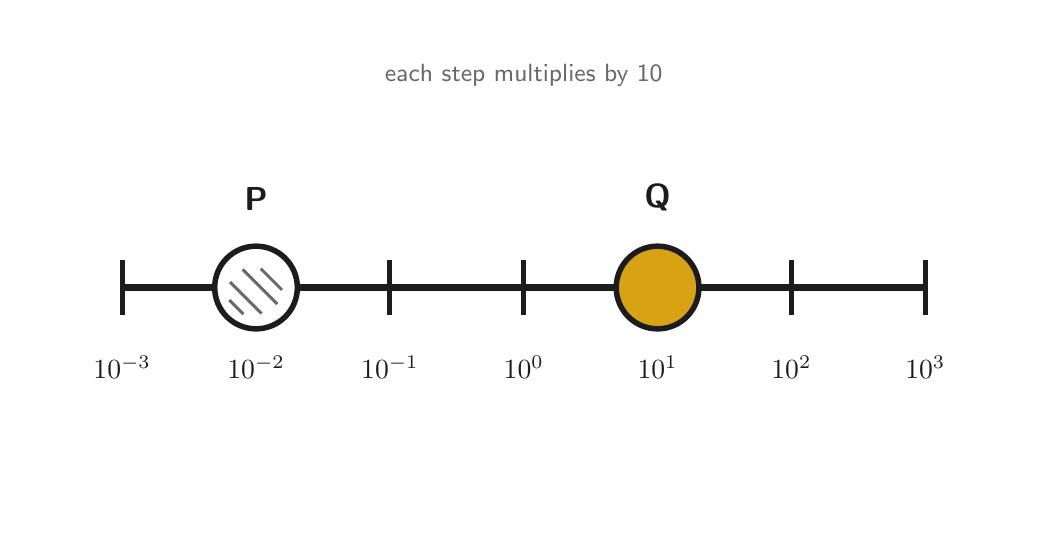
\begin{tikzpicture}[x=1cm,y=1cm]
  \path[fc canvas] (-.45,-.45) rectangle (12.15,5.95);
  \node[fc small label] at (5.85,5.35) {each step multiplies by 10};

  \draw[draw=fcInk, line width=.85mm] (.75,2.65) -- (10.95,2.65);
  \foreach \x/\e in {.75/-3,2.45/-2,4.15/-1,5.85/0,7.55/1,9.25/2,10.95/3} {
    \draw[draw=fcInk, line width=.62mm] (\x,2.3) -- (\x,3.0);
    \node[font=\bfseries\normalsize, text=fcInk, below=4mm] at (\x,2.3) {$10^{\e}$};
  }

  \node[circle, draw=fcInk, fill=white, line width=.7mm,
    minimum size=10.5mm] at (2.45,2.65) {};
  \draw[draw=fcMuted, line width=.38mm]
    (2.11,2.49) -- (2.29,2.31)
    (2.12,2.72) -- (2.52,2.32)
    (2.28,2.88) -- (2.72,2.44)
    (2.51,2.89) -- (2.78,2.62);
  \node[fc label, above=5mm] at (2.45,3.0) {P};

  \node[circle, draw=fcInk, fill=fcGold, line width=.7mm,
    minimum size=10.5mm] at (7.55,2.65) {};
  \node[fc label, above=5mm] at (7.55,3.0) {Q};
\end{tikzpicture}
\end{document}
